\section{О стабилизации положения равновесия перевернутого маятника.} \label{p14}

Рассмотрим задачу о стабилизации математического маятника в верхнем неустойчивом положении за счет момента $U,$ приложенного на его оси, при этом имеется возможность измерить лишь отклонение маятника от вертикали без его производной или угловой скорости [].

Обозначим угол отклонения $\varphi.$ Нормируя, если нужно, соответствующим образом масштабы времени, координат, уравнения возмущенного движения можно записать в виде

\begin{equation} \label{1.45'}
\frac{d \varphi}{dt} = \psi, \quad \frac{d \psi}{dt} = sin \varphi + U
\end{equation}

Сигнал обратной связи измеряется в виде $y = sin \varphi$. Эта задача решалась в работе \cite{krasovsk63} нахождением закона регулирования $$\frac{d U}{d t} = a U(t) + \int_{t - h}^{t} (a (\tau g (\tau) + b U (\tau))) d \tau.$$

Найден стабилизирующий закон регулирования в виде уравнения

\begin{equation} \label{1.46'}
\begin{array}{c}
\displaystyle \frac{d U}{d t} = - 4,6116 \varphi (t) - 3,1974 u(t) -\\
\displaystyle - 4,6116 \int_{t - 1}^{t} (7,358 ch(t + s) + 4,329 sh(t + \tau)) \varphi (t) +\\
\displaystyle + u(\tau) \int_{t - 1}^{t + \tau} (7,358 ch(s + t) + 4,328 sh(s + t)) sh(s - r) ds) d \tau
\end{array}
\end{equation}

Этот закон управления представляется достаточно сложным. Покажем, что рассматриваемая задача о стабилизации решается управлением вида 

\begin{equation} \label{1.47'}
U = - a \sin \varphi (t) - \int_{t-h}^{t} L e^{ b (\tau - t)} (\sin \varphi (t) - \sin \varphi (\tau)) d \tau \cos (\varphi(t))
\end{equation}

где $a$, $b$ и $L$ есть некоторые искомые постоянные $a > 1, \ b, L > 0$

Введем функционал $$V = \frac12 \psi ^ 2 (t) + (a - 1) (1 - \cos \varphi (t)) + \frac12 \int_{t-h}^{t} L e^{b (\tau - t)} (\sin \varphi(t) - \sin \varphi (\tau))^2 d \tau$$

Несложно видеть, что он является определенно-положительным, допускающим бесконечно малый высший предел относительно $\varphi = \varphi (t)$ и $\psi = \psi (t)$

Для его производной находим оценку
$$
\begin{array}{c}
\displaystyle \dot V = \psi (t) (\sin \varphi (t) - a \sin \varphi (t) -\\
\displaystyle - L \int_{t-h}^{t} e^{b (\tau - t)} (\sin \varphi (t) - \sin \varphi (\tau)) d \tau \cos \varphi (t)) + (a - 1) \sin \varphi (t) \psi (t)-\\
\displaystyle - \frac12 b e^{- L h} (\sin \varphi (t) - \sin \varphi (t - h))^2 + \cos \varphi (t) \int_{t-h}^{t} L e^{b (\tau - t)} (\sin \varphi (t)-\\
\displaystyle - \sin \varphi (\tau)) d \tau - \frac12 b L \int_{t-h}^{t} e^{b (\tau - t)} (\sin \varphi (t) - \sin \varphi (\tau))^2 d \tau =\\
\displaystyle = - \frac12 b e^{- L h} (\sin \varphi (t) - \sin \varphi (t - h))^2 - \frac12 b L \int_{t-h}^{t} e^{L (\tau - t)} (\sin \varphi (t) - \sin \varphi (\tau))^2 d \tau \le 0
\end{array}
$$

Множество $\{ \dot V = 0 \}$ может содержать лишь движения $\psi (t) = const,$ или $\dot \psi \equiv 0, \quad \varphi = \pi k, \quad k \in Z$

Соответственно, получаем, что управление (\ref{1.47'}) решает поставленную задачу о стабилизации.

Проведем численный анализ управлений (\ref{1.46'}) и (\ref{1.47'}) при $a = 1.1, L = 1, b = 0.8, h = 1$

\begin{figure}[h]
	\centering
	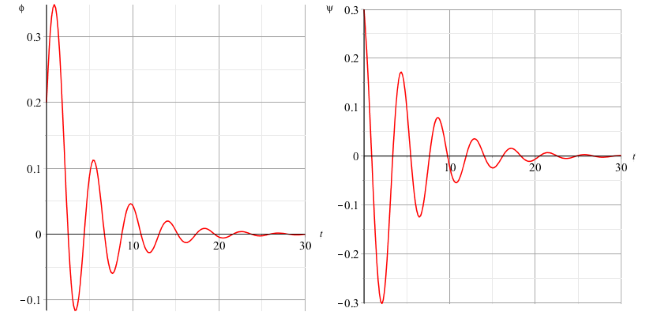
\includegraphics{pendulum}
	\caption{Результаты моделирования при управлении (\ref{1.47'})}
	\label{fig:pendulum_1}
\end{figure}
